% The main file for developing the proposal. 
% Variants with different class options are 
% - submit.tex (no draft stuff, no ednotes, no revision information)
% - public.tex (like submit.tex, but no financials either) 
\providecommand{\classoptions}{,keys} % to be overwritten in variants
\documentclass[noworkareas,deliverables,gitinfo,report,propB\classoptions]{euproposal}
\usepackage[T1]{fontenc}
\usepackage[utf8]{inputenc}
\addbibresource{../lib/dummy}
%%% institutions
\WAinstitution[id=PS,
        countryshort=FR,
        acronym=UPSud]
        {Universit\'e Paris-Sud}

\WAinstitution[id=LL,
        countryshort=FR,
        acronym=Logilab]
        {Logilab}

\WAinstitution[id=UV,
        countryshort=FR,
        acronym=UVSQ]
        {Universit\'e de Versailles Saint-Quentin}

\WAinstitution[id=UJF,
        countryshort=FR,
        acronym=UGA]
        {Universit\'e Grenoble Alpes}

\WAinstitution[id=UB,
        countryshort=FR,
        acronym=CNRS]
        {CNRS}

\WAinstitution[id=UO,
        countryshort=UK,
        acronym=UOXF]
        {University of Oxford}

\WAinstitution[id=USH,
        countryshort=UK,
        acronym=USFD]
        {University of Sheffield}

\WAinstitution[id=USO,
        countryshort=UK,
        acronym=SOUTHAMPTON]
        {University of Southampton}

\WAinstitution[id=SA,
        countryshort=UK,
        acronym=USTAN]
        {University of St Andrews}

\WAinstitution[id=UW,
        countryshort=UK,
        acronym=UWarwick]
        {University of Warwick}

\WAinstitution[id=JU,
        countryshort=DE,
        acronym=JacobsUni]
        {Jacobs University Bremen}

\WAinstitution[id=FAU,
        countryshort=DE,
        acronym=FAU]
        {Friedrich-Alexander Universit\"at Erlangen/N\"urnberg}

\WAinstitution[id=UK,
        countryshort=DE,
        acronym=UNIKL]
        {University of Kaiserslautern}

\WAinstitution[id=US,
        countryshort=PL,
        acronym=USlaski]
        {University of Silesia}

\WAinstitution[id=ZH,
        countryshort=CH,
        acronym=UZH]
        {Universit\"{a}t Z\"{u}rich}

\WAinstitution[id=SR,
        countryshort=NO,
        acronym=Simula]
        {Simula Research Laboratory}

\WAinstitution[id=UG,
	countryshort=BE,
	acronym=UGent]
	{Ghent University}

\WAinstitution[id=XFEL,
        countryshort=DE,
        acronym=XFEL]
        {European XFEL GmbH}

% \WAinstitution[id=UWS,
%         countryshort=US,
%         acronym=UWS]
%         {University of Washington at Seattle}

% \WAperson[id=miko, 
%            personaltitle=Prof. Dr.,
%            birthdate=13. September 1964,
%            academictitle=Professor of Computer Science,
%            affiliation=jacu,
%            department=case,
%            privaddress=None of your business,
%            privtel=that neither,
%            email=m.kohlhase@jacobs-university.de,
%            workaddress={Campus Ring 1, 28757 Bremen},
%            worktel=+49 421 200 3140,
%            worktelfax=+49 421 200 3140/493140,
%            workfax=+49 421 200 493140]
%            {Michael Kohlhase}

\WAperson[id=thiery,
           personaltitle=Prof. ,
           birthdate=28 Mai 1973,
           academictitle=Professor of Computer Science,
           affiliation=PS,
           department=Laboratoire de Recherche en Informatique,
           privaddress=None of your business,
           privtel=that neither,
           email=Nicolas.Thiery@u-psud.fr,
           workaddress={Campus Ring 1, 28757 Bremen},
           %worktel=+33 6 77 90 32 79,
           worktelfax=+33 6 77 90 32 79,
           %workfax=N/A
           ]
           {Nicolas M. Thiéry}

%%% Local Variables: 
%%% mode: latex
%%% TeX-master: "proposal"
%%% End: 

% LocalWords:  WAperson miko personaltitle academictitle privaddress privtel Sud
% LocalWords:  workaddress worktel workfax gc worktelfax pcg pcsa WAinstitution
% LocalWords:  shortname partof streetaddress townzip countryshort efo 3kd89
% LocalWords:  jacobs-logo.png Seefahrtstrasse Kruislann Montparnasse Universit
% LocalWords:  baz Westerfield
% Some sections of the included files depend on this.

\begin{document}
\begin{center}\color{red}\huge
  This mock proposal is just an example for \texttt{euproposal.cls} it reflects the ICT
  template of January 2012
\end{center}
\begin{proposal}[site=jacu,jacuRM=36,
  site=efo,efoRM=36,
  site=bar,barRM=36,
  site=baz,bazRM=36,
  coordinator=miko,
  acronym={iPoWr},
  acrolong={\underline{I}ntelligent} {\underline{P}r\underline{o}sal} {\underline{Wr}iting},
  title=\pn: \protect\pnlong,
  callname = ICT Call 1,
  callid = FP7-???-200?-?,
  instrument= Small or Medium-Scale Focused Research Project (STREP), 
  challengeid = 4,
  challenge = ICT for EU Proposals,
  objectiveid={ICT-2012.4.4}, 
  objective = Technology-enhanced Documents,
  outcomeid = b1,
  outcome = {More time for Research, not Proposal writing},
  coordinator=miko,
  months=24,
  compactht]
\begin{abstract}
  Writing grant proposals is a collaborative effort that requires the integration of
  contributions from many individuals. The use of an ASCII-based format like {\LaTeX}
  allows to coordinate the process via a source code control system like
  {\textsc{Subversion}}, allowing the proposal writing team to concentrate on the contents
  rather than the mechanics of wrangling with text fragments and revisions.
\end{abstract}

\tableofcontents

\begin{todo}{from the proposal template}
  Recommended length for the whole part B: 50--60 pages (including tables, references,
  etc.)
\end{todo}
\chapter{Scientific and Technical Quality}\label{chap:quality}
\begin{todo}{from the proposal template}
  Maximum length for the whole of Section 1 –-- twenty pages, not including the tables in
  Section 1.3
\end{todo}

\section{Targeted breakthrough and long-term vision}\label{sec:objectives}
\begin{todo}{from the proposal template}
  Describe the breakthrough(s) that you are targeting to achieve. What is the long-term
  vision (scientific, technological, societal, other) that motivates this breakthrough?
  Explain how this breakthrough is an essential step towards the achievement of your
  long-term vision, in particular in terms of new forms and uses of information and
  information technologies. Describe the concrete objectives that you consider to
  constitute the proof-of-concept of such a breakthrough. The objectives should be those
  that you consider achievable within the project, in spite of the inherent risks. They
  should be stated in a verifiable form, including through the milestones that will be
  indicated under Section 1.3 below.
\end{todo}

%%% Local Variables: 
%%% mode: latex
%%% TeX-master: "propB"
%%% End: 

\section{Novelty and foundational character}\label{sec:progress}
\begin{todo}{from the proposal template}
  Describe the state-of-the-art in the area(s) concerned, and the advance that the
  proposed project would bring about. Clearly describe the novelty of your proposal. In
  what way do you challenge current thinking or assumptions? Novelty should come from new
  ideas, not from the incremental refinement of existing approaches. It can also come from
  new and unexpected combinations of insights from various disciplines. What is the
  scientific foundation that you aim to develop and what are the specific contributions to
  science and technology that your project will make (including in case of failure)?
\end{todo}

%%% Local Variables: 
%%% mode: latex
%%% TeX-master: "propB"
%%% End: 

\section[S/T Methodology]{S/T Methodology\footnote{Note that, whereas the scientific and technological methodology is evaluated
under the criteria ‘S/T quality’, the quality of the
actual workplan is evaluated under FET-Open under the criteria ‘Implementation’.}}\label{sec:methodology}
\begin{todo}{from the proposal template}
Provide a detailed description of the scientific and technological approach or methodology
by which you will attempt to reach your objectives. Demonstrate that you are aware of the
level and nature of the risks of failure, and that you have a good idea on how to address
these risks. Describe a progression of crucial milestones and decision points for your
project, and their expected timing. What would constitute success? What would you learn
from an eventual failure? Where relevant, show how your approach takes into account the
difficulties inherent to the multi-disciplinary nature of the idea or approach that you
are proposing. 
 A detailed work plan should be presented, broken down into work
packages\footnote{A work package is a major sub-division of the proposed project with a
  verifiable end-point – normally a deliverable or an important milestone in the overall
  project.} (WPs) which should follow the logical phases of the implementation of the
project, and include consortium management and assessment of progress and results. (Note
that your overall approach to management will be described later, in Section 2).

Notes: The number of work packages used must be appropriate to the complexity of the work
and the overall value of the proposed project. The planning should be sufficiently
detailed to justify the proposed effort and allow progress monitoring by the Commission.

\end{todo}
\newpage\begin{todo}{from the proposal template}
\begin{enumerate}
\item Describe the overall strategy of the work plan\ednote{Maximum length – one page}
\item Show the timing of the different WPs and their components (Gantt chart or similar).
\end{enumerate}
\end{todo}
\begin{figure}
  \caption{Work package dependencies}
  \label{fig:wp-deps}
\end{figure}

\ganttchart[draft,xscale=.45] 

%%% Local Variables: 
%%% mode: LaTeX
%%% TeX-master: "propB"
%%% End: 

% LocalWords:  workplan.tex ednote wp-deps ganttchart xscale


\newpage
\subsection{Work Package List}\label{sec:wplist}

\begin{todo}{from the proposal template}
Please indicate one activity per work package:
RTD = Research and technological development; DEM = Demonstration; MGT = Management of the consortium
\end{todo}

%\makeatletter\wp@total@RM{management}\makeatother
\wpfig[pages,type]

\newpage\subsection{List of Deliverables}\label{sec:deliverables}

\begin{todo}{from the proposal template}
\begin{compactenum}
\item Deliverable numbers in order of delivery dates. Please use the numbering convention <WP number>.<number of deliverable within
that WP>. For example, deliverable 4.2 would be the second deliverable from work package 4.
\item Please indicate the nature of the deliverable using one of the following codes:
R = Report, P = Prototype, D = Demonstrator, O = Other
\item Please indicate the dissemination level using one of the following codes:
PU = Public
PP = Restricted to other programme participants (including the Commission Services).
RE = Restricted to a group specified by the consortium (including the Commission Services).
CO = Confidential, only for members of the consortium (including the Commission Services).
\end{compactenum}
\end{todo}
We will now give an overview over the deliverables and milestones of the work
packages. Note that the times of deliverables after month 24 are estimates and may change
as the work packages progress.

In the table below, {\emph{integrating work deliverables}} (see top of
section~\ref{sec:wplist}) are printed in boldface to mark them. They integrate
contributions from multiple work packages. \ednote{CL: the rest of this paragraph does not
  comply with the EU guide for applicants, needs to be rewritten}These can have the
dissemination level ``partial'', which indicates that it contains parts of level
``project'' that are to be disseminated to the project and evaluators only. In such
reports, two versions are prepared, and disseminated accordingly.

{\footnotesize\inputdelivs{8cm}}


%%% Local Variables: 
%%% mode: latex
%%% TeX-master: "propB"
%%% End: 

\newpage\subsection{List of Milestones}\label{sec:milestones}

\begin{todo}{from the proposal template}
  Milestones are control points where decisions are needed with regard to the next stage
  of the project. For example, a milestone may occur when a major result has been
  achieved, if its successful attainment is a requirement for the next phase of
  work. Another example would be a point when the consortium must decide which of several
  technologies to adopt for further development.

  Means of verification: Show how you will confirm that the milestone has been
  attained. Refer to indicators if appropriate. For examples: a laboratory prototype
  completed and running flawlessly, software released and validated by a user group, field
  survey complete and data quality validated.
\end{todo}


The work in the {\pn} project is structured by seven milestones, which coincide with the
project meetings in summer and fall.  Since the meetings are the main face-to-face
interaction points in the project, it is suitable to schedule the milestones for these
events, where they can be discussed in detail. We envision that this setup will give the
project the vital coherence in spite of the broad mix of disciplinary backgrounds of the
participants.\ednote{maybe automate the milestones}

\begin{milestones}
  \milestone[id=kickoff,verif=Inspection,month=1]
    {Initial Infrastructure}
    {Set up the organizational infrastructure, in particular: Web Presence, project TRAC,\ldots}
  \milestone[id=consensus,verif=Inspection,month=24]{Consensus} {Reach Consensus on the
    way the project goes}
  \milestone[id=exploitation,verif=Inspection,month=36]{Exploitation}{The exploitation
    plan should be clear so that we can start on this in the last year.}
  \milestone[id=final,verif=Inspection,month=48]{Final Results}{all is done}
\end{milestones}

%%% Local Variables: 
%%% mode: latex
%%% TeX-master: "propB"
%%% End: 

% LocalWords:  pn ednote verif ldots


\subsection{Work Package Descriptions}\label{sec:workpackages}
\begin{workplan}
\begin{workpackage}[id=management,type=MGT,wphases=0-24!.2,
  title=Project Management,short=Management,
  jacuRM=2,barRM=2,efoRM=2,bazRM=2,lead=jacu,status=canceled]
We can state the state of the art and similar things before the summary in the boxes
here. 
\wpheadertable
\begin{wpobjectives}
  \begin{itemize}
    \item To perform the administrative, scientific/technical, and financial
      management of the project
    \item To co-ordinate the contacts with the EU
    \item To control quality and timing of project results and to resolve conflicts
    \item To set up inter-project communication rules and mechanisms
  \end{itemize}
\end{wpobjectives}

\begin{wpdescription}
  Based on the Consortium Agreement, i.e. the contract with the European Commission, and
  based on the financial and administrative data agreed, the project manager will carry
  out the overall project management, including administrative management.  A project
  quality handbook will be defined, and a {\pn} help-desk for answering questions about
  the format (first project-internal, and after month 12 public) will be established. The
  project management will\ldots we can even reference deliverables:
  \delivref{management}{report2} and even the variant with a title:
  \delivtref{management}{report2}
\begin{tasklist}
  \begin{task}
    To perform the administrative, scientific/technical, and financial management of the
    project
    \end{task}
    \begin{task}
      To co-ordinate the contacts with the EU
    \end{task}
    \begin{task}
      To control quality and timing of project results and to resolve conflicts
    \end{task}
    \begin{task}[status=canceled]
      To set up inter-project communication rules and mechanisms
    \end{task}
  \end{tasklist}
\end{wpdescription}


\begin{wpdelivs}
  \begin{wpdeliv}[due=1,id=mailing,nature=O,dissem=PP,miles=kickoff,lead=jacu]
    {Project-internal mailing lists}
  \end{wpdeliv}
  \begin{wpdeliv}[due=3,id=handbook,nature=R,dissem=PU,miles=consensus,lead=jacu]
    {Project management handbook}
  \end{wpdeliv}
  \begin{wpdeliv}[due=44,id=worldpeace,nature=R,dissem=PU,status=canceled,lead=jacu]
    {Plan to save the world}
  \end{wpdeliv}
\begin{wpdeliv}[due={6,12,18,24,30,36,42,48},id=report2,nature=R,dissem=public,miles={consensus,final}]
  {Periodic activity report} 
  Partly compiled from activity reports of the work package
  coordinators; to be approved by the work package coordinators before delivery to the
  Commission.  Financial reporting is mainly done in months 18 and 36.\Ednote{how about
    these numbers?}
  \end{wpdeliv}
 \begin{wpdeliv}[due=6,id=helpdesk,dissem=PU,nature=O,miles=kickoff,lead=jacu]
    {{\pn} Helpdesk}
  \end{wpdeliv}
  \begin{wpdeliv}[due=36,id=report6,nature=R,dissem=PU,miles=final,lead=jacu]
    {Final plan for using and disseminating the knowledge}
  \end{wpdeliv}
  \begin{wpdeliv}[due=48,id=report7,nature=R,dissem=PU,miles=final,lead=jacu]
    {Final management report}
  \end{wpdeliv}
\end{wpdelivs}
\end{workpackage}

%%% Local Variables: 
%%% mode: LaTeX
%%% TeX-master: "propB"
%%% End: 

% LocalWords:  wp-management.tex workpackage efoRM bazRM wpheadertable pn ldots
% LocalWords:  wpobjectives wpdescription delivref delivtref wpdelivs wpdeliv
% LocalWords:  dissem Ednote pdataRef deliv mansubsusintReport wphases
\newpage
\begin{workpackage}%
[id=dissem,type=RTD,lead=efo,
 wphases=10-24!1,
 title=Dissemination and Exploitation,short=Dissemination,
 efoRM=8,jacuRM=2,barRM=2,bazRM=2]
We can state the state of the art and similar things before the summary in the boxes
here. 
\wpheadertable

\begin{wpobjectives}
  Much of the activity of a project involves small groups of nodes in joint work. This
  work package is set up to ensure their best wide-scale integration, communication, and
  synergetic presentation of the results. Clearly identified means of dissemination of
  work-in-progress as well as final results will serve the effectiveness of work within
  the project and steadily improve the visibility and usage of the emerging semantic
  services.
\end{wpobjectives}

\begin{wpdescription}
  The work package members set up events for dissemination of the research and
  work-in-progress results for researchers (workshops and summer schools), and for
  industry (trade fairs). An in-depth evaluation will be undertaken of the response of
  test-users.

  Within two months of the start of the project, a project website will go live. This
  website will have two areas: a members' area and a public area.\ldots
\end{wpdescription}

\begin{wpdelivs}
  \begin{wpdeliv}[due=2,id=website,nature=O,dissem=PU,miles=kickoff]
     {Set-up of the Project web server}
   \end{wpdeliv}
   \begin{wpdeliv}[due=8,id=ws1proc,nature=R,dissem=PU,miles={kickoff}]
     {Proceedings of the first {\pn} Summer School.}
   \end{wpdeliv}
   \begin{wpdeliv}[due=9,id=dissem,nature=R,dissem=PP]
     {Dissemination Plan}
   \end{wpdeliv}
   \begin{wpdeliv}[due=9,id=exploitplan,nature=R,dissem=PP,miles=exploitation]
     {Scientific and Commercial Exploitation Plan}
   \end{wpdeliv}
   \begin{wpdeliv}[due=20,id=ws2proc,nature=R,dissem=PU,miles={exploitation}]
     {Proceedings of the second {\pn} Summer School.}
   \end{wpdeliv}
   \begin{wpdeliv}[due=32,id=ss1proc,nature=R,dissem=PU,miles={exploitation}]
     {Proceedings of the third {\pn} Summer School.}
   \end{wpdeliv}
   \begin{wpdeliv}[due=44,id=ws3proc,nature=R,dissem=PU,miles=exploitation]
     {Proceedings of the fourth {\pn} Summer School.}
   \end{wpdeliv}
 \end{wpdelivs}
\end{workpackage}

%%% Local Variables: 
%%% mode: LaTeX
%%% TeX-master: "propB"
%%% End: 

% LocalWords:  wp-dissem.tex workpackage dissem efo fromto bazRM wpheadertable
% LocalWords:  wpobjectives wpdescription ldots wpdelivs wpdeliv ws1proc pn
% LocalWords:  exploitplan ws2proc ss1proc ws3proc pdataRef deliv
% LocalWords:  mansubsusintReport
\newpage
\begin{workpackage}[id=class,type=RTD,lead=jacu,
                    wphases=3-9!1,
                    title=A {\LaTeX} class for EU Proposals,short=Class,
                    jacuRM=12,barRM=12]
We can state the state of the art and similar things before the summary in the boxes
here. 
\wpheadertable
\begin{wpobjectives}
\LaTeX is the best document markup language, it can even be used for literate
programming~\cite{DK:LP,Lamport:ladps94,Knuth:ttb84}

  To develop a {\LaTeX} class for marking up EU Proposals
\end{wpobjectives}

\begin{wpdescription}
  We will follow strict software design principles, first comes a requirements analys,
  then \ldots
\end{wpdescription}

\begin{wpdelivs}
  \begin{wpdeliv}[due=6,id=req,nature=R,dissem=PP,miles=kickoff]
     {Requirements analysis}
   \end{wpdeliv}
   \begin{wpdeliv}[due=12,id=spec,nature=R,dissem=PU,miles=consensus]
     {{\pn} Specification }
   \end{wpdeliv}
   \begin{wpdeliv}[due=18,id=demonstrator,nature=P,dissem=PU,miles={consensus,final}]
     {First demonstrator ({\tt{article.cls}} really)}
   \end{wpdeliv}
   \begin{wpdeliv}[due=24,id=proto,nature=P,dissem=PU,miles=final]
     {First prototype}
   \end{wpdeliv}
    \begin{wpdeliv}[due=36,id=release,nature=P,dissem=PU,miles=final]
      {Final {\LaTeX} class, ready for release}
    \end{wpdeliv}
  \end{wpdelivs}
Furthermore, this work package contributes to {\pdataRef{deliv}{managementreport2}{label}} and
{\pdataRef{deliv}{managementreport7}{label}}.
\end{workpackage}

%%% Local Variables: 
%%% mode: LaTeX
%%% TeX-master: "propB"
%%% End: 
\newpage
\begin{workpackage}[id=temple,type=DEM,lead=bar,
  wphases=6-12!1,
  title={\pn} Proposal Template,short=Template,barRM=6,bazRM=6]
We can state the state of the art and similar things before the summary in the boxes
here. 
\wpheadertable

\begin{wpobjectives}
  To develop a template file for {\pn} proposals
\end{wpobjectives}

\begin{wpdescription}
  We abstract an example from existing proposals
\end{wpdescription}

\begin{wpdelivs}
  \begin{wpdeliv}[due=6,id=req,nature=R,dissem=PP,miles=kickoff,lead=bar]
    {Requirements analysis}
  \end{wpdeliv}
  \begin{wpdeliv}[due=12,id=spec,nature=R,dissem=PU,miles=consensus,lead=baz]
    {{\pn} Specification }
  \end{wpdeliv}
  \begin{wpdeliv}[due=18,id=demonstrator,nature=D,dissem=PU,miles={consensus,final},lead=bar]
    {First demonstrator ({\tt{article.cls}} really)}
  \end{wpdeliv}
  \begin{wpdeliv}[due=24,id=proto,nature=P,dissem=PU,miles=final,lead=baz]
    {First prototype}
  \end{wpdeliv}
  \begin{wpdeliv}[due=36,id=release,nature=P,dissem=PU,miles=final,lead=bar]
    {Final Template, ready for release}
  \end{wpdeliv}
\end{wpdelivs}
Furthermore, this work package contributes to {\pdataRef{deliv}{managementreport2}{label}} and
{\pdataRef{deliv}{managementreport7}{label}}.
\end{workpackage}

%%% Local Variables: 
%%% mode: LaTeX
%%% TeX-master: "propB"
%%% End: 

% LocalWords:  wp-temple.tex workpackage fromto pn bazRM wpheadertable wpdelivs
% LocalWords:  wpobjectives wpdescription wpdeliv req dissem tt article.cls
% LocalWords:  pdataRef deliv systemsintReport
\newpage
\end{workplan}
\newpage\subsection{Significant Risks and Associated Contingency Plans}\label{sec:risks}
\begin{todo}{from the proposal template}
  Describe any significant risks, and associated contingency plans
\end{todo}
\begin{oldpart}{need to integrate this somewhere. CL: I will check other proposals to see how they did it; the Guide does not really prescribe anything.}
\paragraph{Global Risk Management}
The crucial problem of \pn (and similar endeavors that offer a new basis for communication
and interaction) is that of community uptake: Unless we can convince scientists and
knowledge workers industry to use the new tools and interactions, we will
never be able to assemble the large repositories of flexiformal mathematical knowledge we
envision. We will consider uptake to be the main ongoing evaluation criterion for the network.
\end{oldpart}

%%% Local Variables: 
%%% mode: latex
%%% TeX-master: "propB"
%%% End: 



%%% Local Variables: 
%%% mode: latex
%%% TeX-master: "propB"
%%% End: 

% LocalWords: workplan newpage wplist makeatletter makeatother wpfig
% LocalWords:  workpackages wp-dissem wp-class wp-temple

%%% Local Variables: 
%%% mode: LaTeX
%%% TeX-master: "propB"
%%% End: 

\newpage
\section{Implementation}\label{sec:impl}
The implementation of in-situ computation is organized along the information model outlined in
the last section.
It is realized as a set of Javascript modules in the JOBAD framework~\cite{JOBAD:on}, a Javascript framework for instrumenting (active) documents with user interactions; see~\cite{GLR:WebSvcActMathDoc09} for details.

We will first discuss unit conversion (see Section~\ref{sec:ex:units}) as a special case of in-situ computation and then generalize to the case of a non-trivial context and generalize to arbitrary computations in Section~\ref{sec:impl:general}.

\subsection{Unit Conversion}\label{sec:impl:units}
Unit conversion is a special case of in-situ computation, because
\begin{compactitem}
\item the computations are essentially limited to unit conversion and
\item context is trivial, since the computational objects -- the quantity expressions -- consist only of a number and a unit expression. The units are all defined constants and local identifiers do not exist.
\end{compactitem}
Ulrich Rabenstein of the KWARC group has implemented a semantics extraction procedure that finds quantity expression in HTML5 documents, analyzes their content structure and represents them in content MathML and stored as (standoff) RDF annotations.
These can be used to feed in-situ computations.

The user interface for unit conversion can be implemented directly in JOBAD by delegating the conversion (the content MathML representation of the quantity expressions has sufficient information) to a unit converter -- we use the units package from Astropy~\cite{astropy}, an extendible python library for astronomy -- whose result can be converted to Presentation MathML for inclusion in the document.
We show the user interaction here.

Before starting to convert something, the user can highlight all quantity expressions in a given document.
This results in a document, as shown in Figure~\ref{fig:highlight}.
We further use this snippet as an example.

\begin{figure}[ht]
    \fbox{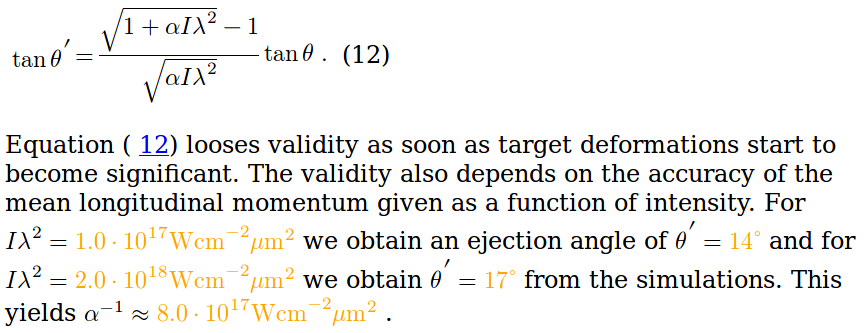
\includegraphics[width=\textwidth]{screenshots/highlight}}
    \caption{Highlighting Quantity Expressions in \cite{physics/9807021}}\label{fig:highlight}
\end{figure}

In the first case, the user wants to convert a unit in just one expression to an equivalent one, say watt to horsepower.
For that, she can right-click on this particular expression and choose a target unit (e.g.  horsepower) from the list of units that are equivalent to Watt.
Figure~\ref{fig:convertone} demonstrates this and Figure~\ref{fig:convertoneresult} displays the result of the computation.

\begin{figure}
  \begin{subfigure}{\textwidth}
    \fbox{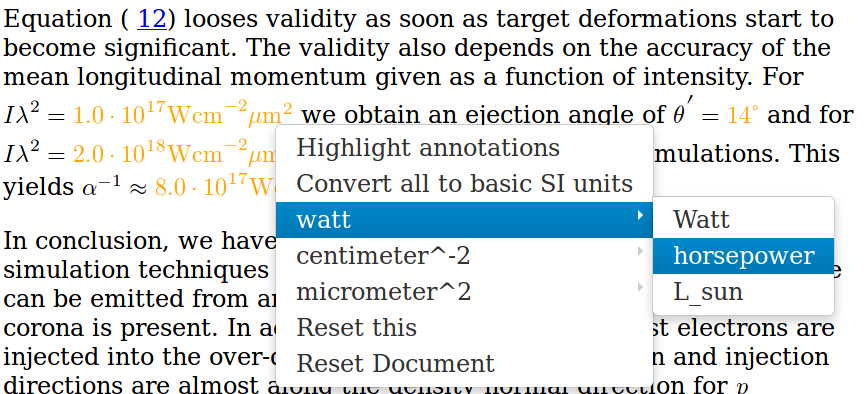
\includegraphics[width=\textwidth]{screenshots/convertone}}
    \caption{Choosing A Target Unit}\label{fig:convertone}
    \fbox{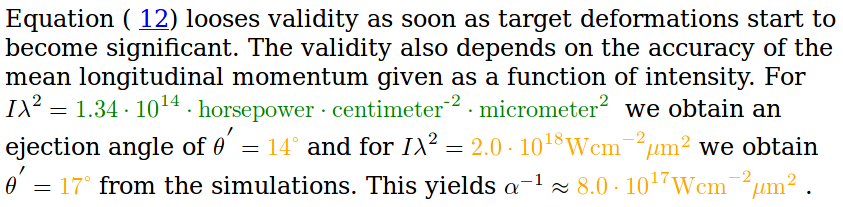
\includegraphics[width=\textwidth]{screenshots/convertoneresult}}
    \caption{The Result of converting one QE}\label{fig:convertoneresult}
    \fbox{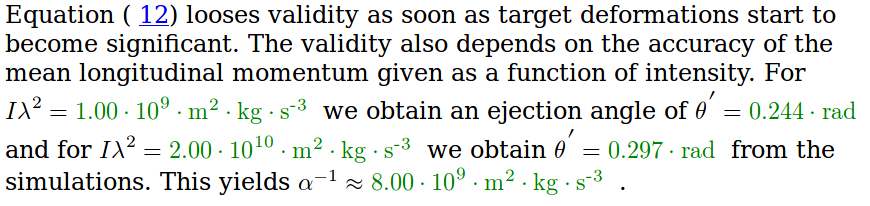
\includegraphics[width=\textwidth]{screenshots/si}}
    \caption{Converting a Document To SI}\label{fig:si}
  \end{subfigure}
  \caption{In-Situ Unit Conversion}\label{fig:unit-conversion}
\end{figure}

The current example only allows local conversions, but of course the user also wants to convert units document-wide -- ideally from one system of measurement to another.
Figure~\ref{fig:si} shows the result of a prototypical implementation, which converts all units to irreducible SI base units.
This could, for instance, be extended to automatically convert all quantity expressions in a document from imperial to metric units and vice versa.

\subsection{A General Framework for In-Situ Computation}\label{sec:impl:general}

In addition to the example above, we have also implemented a prototype of the general in-situ computation manager detailed above.
A right click on a formula $F$ triggers the JOBAD menu, which has an ``Active Computation'' field.

  \begin{itemize}
  \item First, the \textbf{context extractor}, a function that for all the \lstinline|ci| elements in the content formula $C$ associated with $F$, and tries to find the associated variable declarations by going up the parent chain of $F$ and the symbol declarations from the home theory.
  Note that using the content MathML representation $C$ of $F$ gets us around disambiguation problems: even if the presentation of $F$ is ambiguous (e.g. by using variable or constant names multiple times), $C$ is not.
  \item The variable context is displayed to the user prompting instantiation in a popup form: the \textbf{in-situ computation manager} (see Figure~\ref{fig:compman}, which allows to give values for the components of the equation, pick different actions (simplification, equation solving, \ldots ) and ways of providing the results (in-place, footnote, \ldots ).
  As the current system is only a prototype, one can currently only select the Evalutation Action.
  \item In a second step, the  user-supplied values are parsed into content MathML, inserted into $C$, yielding the content MathML expression $C'$, which is then shipped to the computational engine.
  Currently we only support the MMT system as a computational engine, but this is not a restriction, since MMT can delegate computations to engines like GAP, Sage, PARI, \ldots via the SCSCP protocol~\cite{ODK-D3.3}.
  \item Finally, the result $R$ of computing $C'$ -- a content MathML expression -- is inserted back into the original computation context.
  This context can then be presented in presentation MathML and inserted into the document according to the method the user selected \footnote{
  Currently, the system presents the user with the computed context directly. }.
  \end{itemize}

  \begin{figure}[ht]\centering
    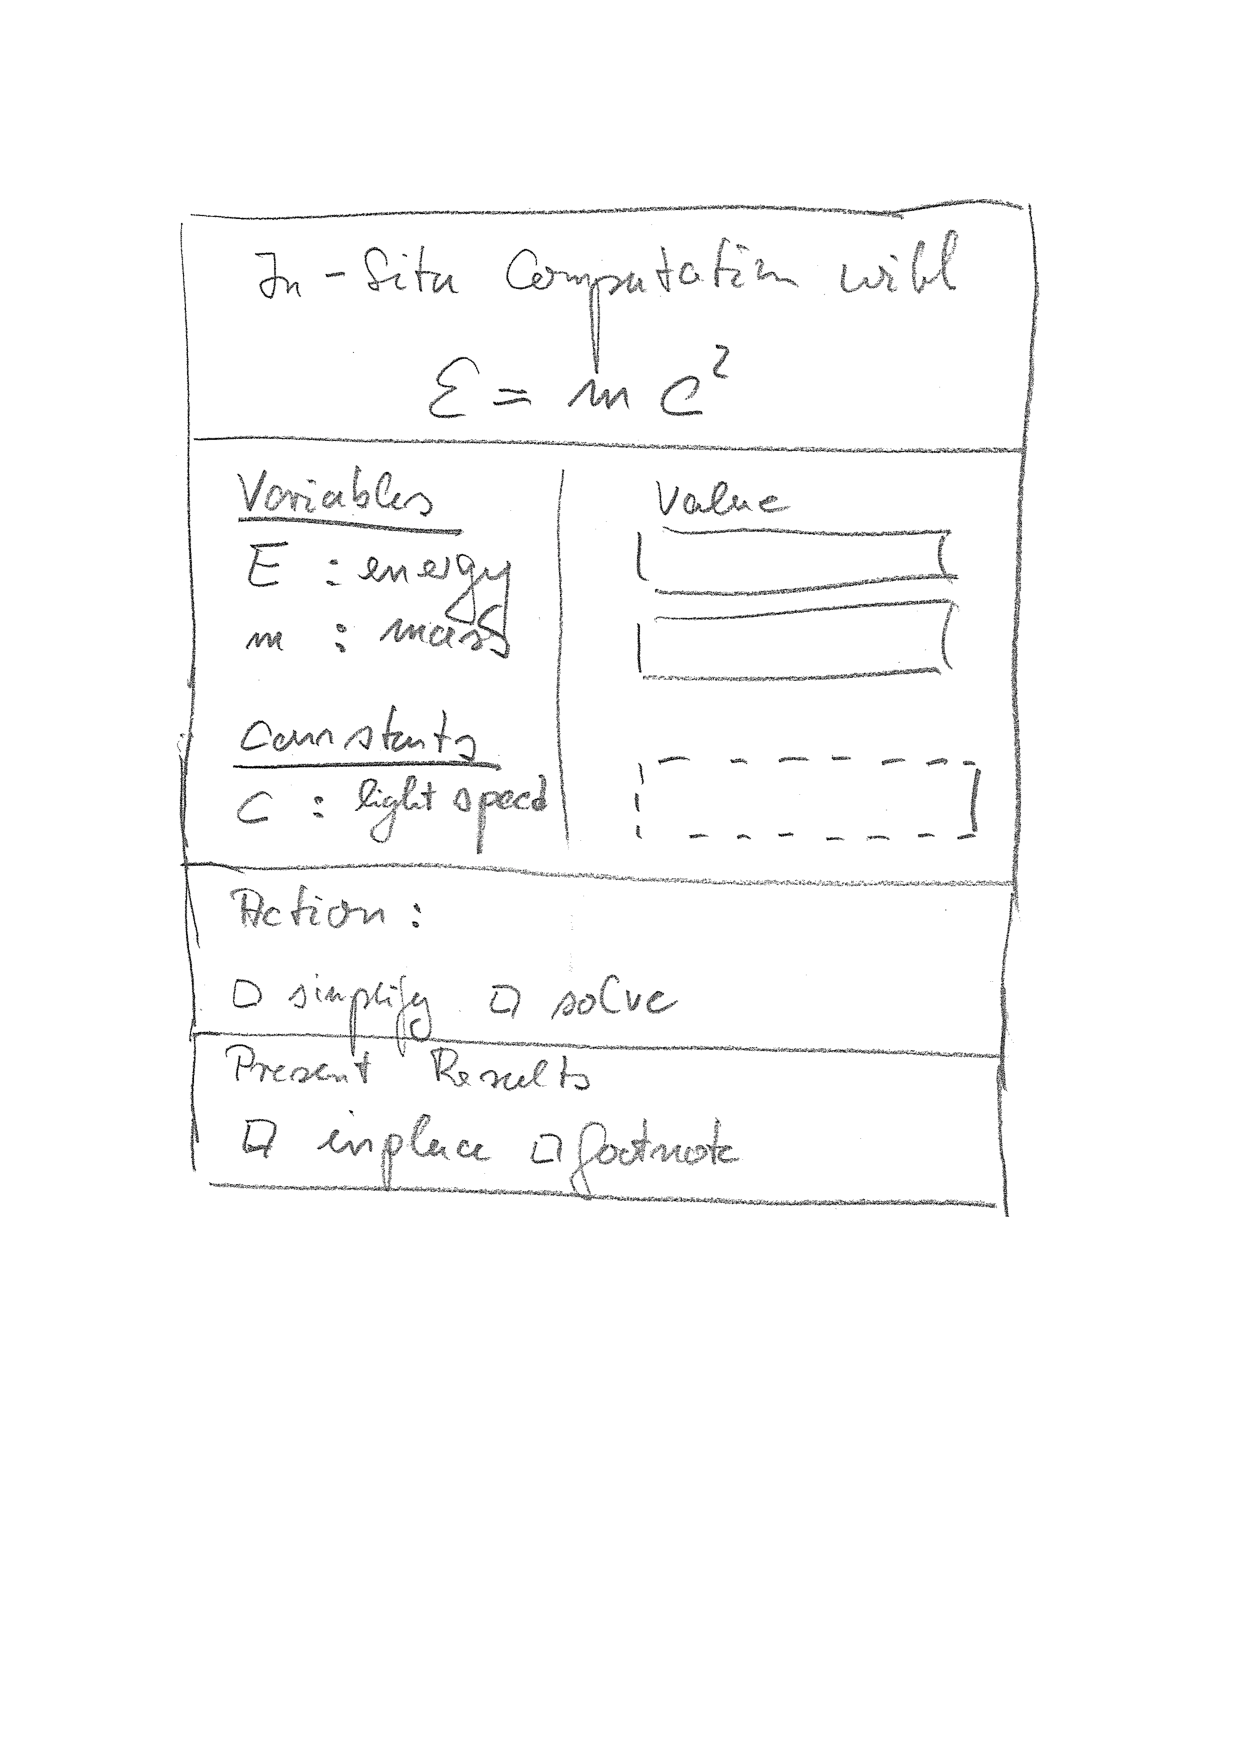
\includegraphics[width=12cm]{screenshots/compman}
    \caption{In-Situ Computation Manager}\label{fig:compman}
  \end{figure}

\subsection{Code Availability, Licensing and Demos}

For both of the examples in this section, an implementation is available under Open Source license terms.
For reasons of lacking MathML support in other browsers, we have only tested these demos in Firefox.

A demo of the unit conversion is available at \url{http://ash.eecs.jacobs-university.de/}.
A user can first select a document and then repeat the procedure detailed above in Section~\ref{sec:impl:units}.
The source code of the demo is available in the repository at \url{https://gl.kwarc.info/urabenstein/Semanticextraction/tree/master/server}.
The server can be executed locally following the steps in the corressponding README file.

A protoype of the General Framework for In-Situ Computation is also availble.
It can be found at \url{http://ash.eecs.jacobs-university.de/prototype/} and shows the basics of the process explained in Section~\ref{sec:impl:general}.
it consists of a frontend component, the source code of which can be found at \url{https://gl.mathhub.info/ODK/ActiveComputationDemo}, as well as a backend component inside the MMT system.
The source code to the backend component can be found at \url{https://github.com/UniFormal/MMT/tree/master/src/mmt-odk/src/info/kwarc/mmt/odk/activecomp}.

%%% Local Variables:
%%% mode: latex
%%% TeX-master: "report"
%%% End:
\newpage
% ---------------------------------------------------------------------------
%  Section 2: Impact
% ---------------------------------------------------------------------------

\TOWRITE{ALL}{Proofread 2 Impact1.4 Ambition pass 2}

\section{Impact}
\label{sec:impact}

%\TOWRITE{Simula}{Hans Petter and Valeriya will make a second iteration on the impact section for Friday}

\TOWRITE{ALL}{Check and complement the impact section}

The project, with its ambitious vision, general and broad approach, and 
challenging work plan, will offer the opportunity to all partners and beyond 
to complement their research expertise with methodologies and tools not 
available at their institutions. It will provide pivotal aspects needed 
for the development of a new generation of high-efficient scientific leaders 
with an open and constructive attitude toward collaborative interdisciplinary 
research and innovation. The diverse nature of the objectives composing the 
project will also be taken into account to design a successful and multiform 
dissemination and exploitation strategy.

\subsection{Expected Impacts}

\eucommentary{Please be specific, and provide only information that applies
to the proposal and its objectives. Wherever possible, use quantified
indicators and targets.\\
Describe how your project will contribute to:\\
-- the expected impacts set out in the work programme, under the relevant topic
(including key performance indicators/metrics for monitoring results and impacts);\\
-- improving innovation capacity and the integration of new knowledge
(strengthening the competitiveness and growth of companies by developing
innovations meeting the needs of European and global markets; and, where
relevant, by delivering such innovations to the markets;\\
-- any other environmental and socially important impacts (if not already
covered above).\\
Describe any barriers/obstacles, and any framework conditions (such as
regulation and standards), that may determine whether and to what extent
the expected impacts will be achieved. (This should not include any risk
factors concerning implementation, as covered in section 3.2.)}

\subsubsection{Impacts as Listed in the Work Programme}

The following Key Performance Indicators (KPI) show how \TheProject  addresses the specific impacts
listed in the work programme. KPIs were thought through by the members
of \TheProject so that they are meaningful, reusable, realistic and easily measurable. The following
qualitative and quantitative indicators are divided into the four aims of \TheProject.
If quantitative indicators are more useful for reporting and internal evaluation, qualitative
indicators will give content for further dissemination and communication purposes,
for example through the project website
\footnote{We will survey mathematical departments
(and relevant members of other departments) 
at the end of each Reporting Period (M18, M36, M48) to gauge the awareness of the 
existence and capabilities of \TheProject and its components, and to collect
statistical data for estimating Key Performance Indicators listed
in the table. The success factor is a positive change between the three surveys.}.

\newenvironment{myaim}[1]
{\noindent{\textbf{#1:}} \begingroup\it}
{\endgroup}

\begin{myaim}{Aim 1}
  Improve the productivity of researchers in pure mathematics and
  applications by promoting collaborations based on mathematical
  software, data, and knowledge.
\end{myaim}

\begin{itemize}
\item Success stories reported as blogposts (Qualitative).
\end{itemize}


\begin{myaim}{Aim 2}
  Make it easy for teams of researchers of any size to set up custom,
  collaborative Virtual Research Environments tailored to their
  specific needs, resources and workflows. The \VREs should support
  the entire life-cycle of computational work in mathematical
  research, from initial exploration to publication, teaching and
  outreach.
\end{myaim}

\begin{itemize}
\item Success stories about \ODK based VRE deployments and
generally speaking adoption of \ODK's components (Qualitative);
\item List of known \ODK based VRE deployments (Quantitative);
\item Number of installs of \ODK's components via platform-specific
  distribution channels: Debian popcon, Arch statistics, installer
  downloads, etc. (Quantitative).
\end{itemize}


\begin{myaim}{Aim 3}
  Identify and promote best practices in computational mathematical
  research including: making results easily reproducible; producing
  reusable and easily accessible software; sharing data in a
  semantically sound way; exploiting and supporting the growing
  ecosystem of computational tools.
\end{myaim}
\begin{itemize}
\item Success stories (Qualitative);
\item Number of PyPI hosted packages for \Sage, and similarly for
  other components (Quantitative);
\item Number of additional systems made interoperable with the
  Math-in-the-Middle architecture, on top of the three for the Month
  36 prototype (Quantitative);
\item Metrics on the scale of the Math-in-the-Middle architecture;
  e.g. number of API CDs generated and number of alignments
  (Quantitative).
\end{itemize}

\begin{myaim}{Aim 4}
  Maximise sustainability and impact in mathematics, neighbouring
  fields, and scientific computing.
\end{myaim}
\begin{itemize}
\item Success stories resulting from dissemination activities such as
  workshops (Qualitative);
\item Statistics on workshops organized and conference presentations
  delivered as part of our dissemination activities, including
  estimates of number of attendees (Quantitative);
\item Number of courses and departments \ODK worked with directly and
  an estimate of how many students this subsequently affected
  (Quantitative).
\end{itemize}

\subsubsection{Improving innovation capacity and the integration of new knowledge}


Innovations developed by the \TheProject project will meet the needs of the
following ecosystem participants:

\begin{compactenum}
\item Device/module vendors: hardware manufacturers, equipment
manufacturers of smartphones, tablets, laptops;
\item Network providers: service providers, network infrastructure
vendors (such as Avaya, Juniper, Extreme, Cisco, et al.);
\item Platform providers;
\item Cloud service providers: Software-as-a-Service,
Platform-as-Service, Infrastructure-as-a-Service;
\item Systeme integrators: end-to-end integration services and
value-added services (such as Accenture, HP, IBM, et al.)
\item End users: research communities; stakeholders in IT, healthcare, 
education, aeronautics, and other areas.
\end{compactenum}
Industrial stakeholders will be directly involved in the project and
the VRE development, so that the tool will be exactly tailored to their
specific needs as well as to the needs of the scientific community.
Moreover, this will allow short time-to-market and will facilitate
the technology uptake.

In the next table we have specified different market needs, and the
ways we will address each of them:

%\begin{flushleft}
\tablehead{}
\begin{longtable}{|m{.30\textwidth}|m{.67\textwidth}|}
\hline
\centering Market needs &
\centering\arraybslash How the project will address these needs\\\hline
Performance gain &
The toolkit will enable its users to combine functionality from several major
open-source mathematical software systems and problem-oriented programming 
languages (including mainstream tools such as Python) in a modern integrated environment) on the majority of currently popular hardware platforms 
and operating systems.
\\\hline
Infrastructure capacity: newly built infrastructures with fast broadband
connections are well positioned for adopting our products &
\TheProject will allow different groups of users to collaborate and work simultaneously on the same document, and
thus providing a considerable gain in efficiency.\\\hline
Low scaling costs &
An open source architecture brings affordability: people and
organisations donate efforts towards common goals, and small organisations can
gain access to equipment and research talents otherwise only affordable by
the largest companies. Resources integration will reduce considerably the
time and the costs of operations.\\\hline
Going beyond limitations of interconnect technology &
An open source architecture enhances creativity due to the potential to
attract best minds from a wide pool of people to solve a problem\\\hline
Enabling new applications and features &
Through a series of connections that will be created between previously
separated tools, and data interoperability, \TheProject will enable new
applications and features. All derived VREs are new applications, with new features.\\\hline
Early time-to-market (TTM): companies are looking for solutions that
would improve the speed at which they can procure services to bypass
traditional information technology departments &
The speed of development will improve tremendously due to the new
collaborative features. Liaising with industrial stakeholders during
the development will allow to deliver a tool the suits their needs in
the best possible way, thus speeding-up the time-to-market and technology 
uptake.\\\hline
Easy-to-use service: first-time experiences are crucial to gain
acceptance &
We will design an ergonomic multi-user web-based graphical user
interface, following web standards to best support a large array of
browsers, including cell phones and tablets. We will explore
opportunities for integration in interactive boards, as an aid for
teaching and collaborative research.
\\\hline
\end{longtable}
%\end{flushleft}

\subsubsection{Other Impacts (Environmental and Socially Important Impacts)}


We start from \Sage's mission statement: ``Creating a viable free open
source alternative to \Magma, \Maple, \Mathematica and \Matlab'' but
need to go beyond that goal, and make \TheProject a new reference
tool, that is deployed across science. To be successful our VREs will
need to provide much more than can be done through closed source
commercial systems. Large scale collaborative development is the key
to this goal, both on software and research, but coordination and
projection of vision is still crucial for success. We will focus on
the young generation, which will constitute its future users, for
example by producing learning materials for the so called ``Generation
Y''. ``Generation Y'' is expected to account for 30\% of the total
projected population in 2025, and will be the key influencer for
change in workplace habits, caused by such features as easy
adaptability to new technologies and social media, commonly attributed
to this generation.  \TOWRITE{??}{May we add some reference to support
  this statement?}

\TOWRITE{AK}{This section needs to be extended} 

\subsubsection{Potential Barriers to Impact}

The following barriers to impact will be addressed and overcome using the mitigation
strategies provided. These are distinct from the risks to project delivery
detailed in Section~\ref{sec:risks}.
\TOWRITE{ALL}{Some other barriers? Maybe lack of contribution from community to OpenDreamKit?}
\paragraph{Table 2.1: Barriers to Impact}
\begin{longtable}{ | p{10cm} | c | }\hline
{\bf Barrier description } & {\bf Risk level }\\\hline \hline
{\bf Users will not use the new VRE environment}       &  High       \\\hline
\multicolumn{2}{| p{.97\textwidth}|}{
{\bf Contingency Plan:}  
A major concern in any proposal of this kind is that the resulting
tools will not be adopted by users. This is a particular concern with
such 'tradition-based' community as mathematicians.  This project has two pathways to tackle this:
(1) \TheProject is based on prior work, which \emph{already} has users;
(2) \TheProject will be integrated into the \Jupyter and \Sage, which \emph{already} have a significant user base;
(3) An end-user group formed at the beginning of the project by the representatives from different disciplines and sectors will provide valuable advice on real user needs throughout the project and assist in providing \TheProject sustainability.

In addition, the project's communication, dissemination, and
exploitation strategy will evolve throughout the project's implementation to
ensure that stakeholder communities are fully aware of the project's
progress, potential benefits, and innovative capacity and are engaged
in the integration of the final results.
}\\\hline
{\bf Dominance of competing frameworks  }  &  Medium        \\\hline 
 \multicolumn{2}{| p{.97\textwidth}|}{
{\bf Contingency plan:}  
  Our strategy is to engage with  users  and attract new users at the very beginning
of the project, understand their requirements and design the domain-specific tools.
An international advisory
board will allow us to coordinate with the related research activities within and outside of Europe
and to promote our framework internationally.}\\\hline
\end{longtable}
\TOWRITE{All and NT}{Is dominance of competing frameworks really an issue? Is there anything out there AS GOOD as OpenDreamKit? Would be good to have more than just one barrier though.}



\subsection{Measures to Maximise Impact}
\TOWRITE{ALL}{go through the section and add specific input, relevant to your organisation on dissemination / exploitation activities}
The overall objectives of the dissemination and exploitation strategy are based on the project's core values, which are to improve the productivity of researchers in mathematics and connected fields by providing them with a unique virtual toolkit for a collaborative research tailored to their needs and requirements both during the project period and after the project completion.

\subsubsection{Dissemination and Exploitation of Results}
\label{subsubsect:dissemination}
\eucommentary{-- Provide a draft 'plan for the dissemination and exploitation
of the project's results'. The plan, which should be proportionate to the
scale of the project, should contain measures to be implemented both during
and after the project.\\
Dissemination and exploitation measures should address the full range
of potential users and uses including research, commercial, investment,
social, environmental, policy making, setting standards, skills and
educational training.\\
The approach to innovation should be as comprehensive as possible,
and must be tailored to the specific technical, market and organisational
issues to be addressed\\
-- Explain how the proposed measures will help to achieve the expected impact of the
project . Provide a draft business plan for financial sustainability as stated in the Part
E of the Specific features for Research Infrastructures of the Horizon 2020 European
Research Infrastructures (including e-Infrastructures) Work Programme 2014-2015.\\
-- Where relevant, include information on how the participants will
manage the research data generated and/or collected during the
project, in particular addressing the following issues:
What types of data will the project generate/collect? What
standards will be used? How will this data be exploited and/or
shared/made accessible for verification and re-use (If data cannot
be made available, explain why)? How will this data be curated and preserved?\\
-- Include information about any open source software used or developed by the
project.\\
You will need an appropriate consortium agreement to manage (amongst other things)
the ownership and access to key knowledge (IPR, data etc.). Where relevant,
these will allow you, collectively and individually, to pursue market opportunities
arising from the project's results.\\
The appropriate structure of the consortium to support exploitation is addressed
in section 3.3. \\
-- Outline the strategy for knowledge management and protection. Include measures to
provide open access (free on-line access, such as the ``green'' or ``gold'' model) to
peer-reviewed scientific publications which might result from the project.\\
Open access publishing (also called 'gold' open access) means that an article is
immediately provided in open access mode by the scientific publisher. The associated costs
are usually shifted away from readers, and instead (for example) to the university or
research institute to which the researcher is affiliated, or to the funding agency supporting
the research.\\
Self-archiving (also called ``green'' open access) means that the published article or the
final peer-reviewed manuscript is archived by the researcher - or a representative - in an
online repository before, after or alongside its publication. Access to this article is often -
but not necessarily - delayed (``embargo period''), as some scientific publishers may wish to
recoup their investment by selling subscriptions and charging pay-per-download/view fees
during an exclusivity period.}


The dissemination and exploitation strategy will be
presented in the dissemination and exploitation plan, prepared by the
Coordinator within \TOWRITE{All}{Add reference to task that produces
  dissemination and exploitation plan} the specifically designed WP
and implemented with the help of all partners. The planned activities
will bear in mind the project's scientific and societal impacts, and
build throughout the project to ensure that stakeholder communities
(1) are fully aware of the project and its potential benefits, (2)
engaged in integration of the VRE in their professional activities,
and (3) contribute to the sustainability and improvement of the
VRE. 

We summarise the dissemination activities
and how they will help to achieve the expected impact among our
stakeholders and target audiences in Table~\ref{table:dissem-plan}.

%% HF got to here reviewing 

%Three types of impact are possible with our dissemination and
%communication activities: (1) people or organizations are informed
%about \TheProject; (2) people or organizations act and use our conclusions
%or results; (3) people or organizations contribute and help to develop
%or improve the research infrastructure. The second form of impact
%supposes that parties understand the messages. The third form supposes
%learning, which is a very high level of impact. In the following table,
%we have listed how the proposed measures will help to achieve the
%expected impact among our stakeholders and target audiences.

\begin{table}
\begin{longtable}{|m{3cm}|m{1cm}| m{.56\textwidth} | m{2cm}|}\hline
Dissemination goal &
Target audience&
Dissemination method &
Timeframe and frequency  \\\hline
Project identity and profile &
T1-T6
&
Website; flyers/leaflets; videos.
& 
Throughout project, continuous \\\hline
Broad dissemination &
T3, T4, T6, T7 
&
Biannual e-newsletters; press releases; information database; social networks and platforms; news  in Nature and other editions in other disciplines; lectures in high schools led by PhD students.
& 
Throughout project, quarterly \\\hline
Knowledge transfer, information exchange&
T1,T2, T3
&

Organisation of 10 technical workshops; 10 scientific trainings/year; training of at least 100 PhD students for the infrastructure usage; publications in social aspects; software demonstration during conferences; workshop for PhD students in Africa; participation at the workshop 'Sage and women' in US; participation in international conferences like FPSAC, ISSAC, or the international congress of mathematical software; regular participation in annual Python conference; organising at least 8 scientific trainings for other scientific communities/projects; news  in Nature and other editions in other disciplines; certification by technology clusters.
& 
Throughout project, continuous  \\\hline
Demonstration of advantages and possible applications &
T1-T4
&
Organisation of 10 technical workshops; participation in annual Python conference.
& 
Biannually \\\hline
Uptake of the VRE by new users &
T2-T4
&
White papers; organise at least 8 scientific trainings for other scientific communities/projects; presentation at international conferences; 5 MooCs designed to master students; integration of project results into Master courses and into teacher training courses.
& 
Mo24-, at relevant milestones \\\hline
Sustainable development beyond the project &
T1-T4
&
Policy events; white papers; participation at conferences.
& 
Mo24-, at relevant milestones \\\hline
\end{longtable}

\smallskip
{\bf Key for the ``Target Audience'' column:}
\begin{compactenum}
\item[T1] Scientific community in mathematics and related fields 
     (experienced researchers, under-/graduate/post-graduate students);
\item[T2] Scientific community in other disciplines;
\item[T3] Other relevant European and national initiatives and projects;
\item[T4] Industrial end-users;
\item[T5] Standardisation agencies;
\item[T6] Civil society;
\item[T7] Public at large.
\end{compactenum}
\caption{\label{table:dissem-plan}Dissemination and exploitation plan}
\end{table}

%
%\begin{flushleft}
%\tablehead{}
%\begin{longtable}{|m{2cm}|m{8cm}|l|l|l|}
%\hline
%
%Target users &
%Measures during the project &
%\multicolumn{3}{m{3.9129999cm}|}{Expected impact}\\\hline
% &
% &
%(1) &
%(2) &
%(3)\\\hline
%Scientific community in mathematics
%
%(experienced researchers and PhD students) &
%\begin{compactenum}
%\item Recruitment for the project of specialists from industrial sector
%and PhD students that are already a part of the community ;\item 10
%technical workshops organised in the frame of \TheProject, \item 10
%publications in (social aspects) \item Software demonstration during
%the conferences{\textgreater}publication\item 100 PhD students trained
%and accessing the infrastructure\item Workshops for PhD students in
%Africa
%\end{compactenum}
% &
%X
%
%X
%
%X
%
%X &
%X
%
%X
%
%X
%
%X
%
%X
%
%X
%
%X &
%X
%
%X
%
%X
%
%X
%
%X
%
%X\\\hline
%Scientific community in other disciplines &
%\begin{compactenum}
%\item Direct implication of the representatives of those disciplines
%into the project;\item Annual participation in Pycon international
%conference\item X scientific trainings to other communities; \item News
%in Nature and other editions in other disciplines (specify!)\item Up to
%X PhD students trained on the tool in biology, physics etc.\item
%Workshop ``~sage \& women~'' in USA{\textgreater} pour
%IPython
%\end{compactenum}
% &
%X
% &
%X
%X
%X
%X
%X
%X
% &
%X
%X
%X\\\hline
%Policy makers &
%Are not directly concerned by the tool, but can be informed via
%international conferences and publications &
%X &
% &
%\\\hline
%Industry &
%\begin{compactenum}
%\item Industrial stakeholders have common needs with academic
%researchers. They bring to the project their specific competences and
%human resources. They are actively involved into the workshops and
%trainings (50\% of audience). The project aims the enlargement of the
%community thanks notably to new industrial actors (including in other
%disciplines and sectors). They will appropriate the tool by their
%direct involvement into the project, by participation to the workshops,
%trainings and conferences or by their usual information channels.\item
%Annual participation in Pycon international conference\item
%Certification by technology clusters
%\end{compactenum}
% &
%X &
%X
%X
%X
% &
%X\\\hline
%Standartisation
%
%agencies  &
%\begin{compactenum}
%\item At the end of the project,~after internal standartisation, the new
%norms will be accorded with specialised agencies at national and EU
%levels
%\end{compactenum}
% &
% &
%X &
%\\\hline
%Students &
%\begin{compactenum}
%\item 5 MooCs destined to master students.\item The tool will be used
%for the elaboration of pedagogical documents, referenced on the
%specific website\item The projects results will be integrated into
%Master courses, and into teacher training courses
%\end{compactenum}
% &
%X
%X
%X
% &
%X
%X &
%\\\hline
%Civil society &
%\begin{compactenum}
%\item Results will be presented on the annual event “Worldwide meetings
%of the free software”. This event generally touches upon all free
%phenomena in the society, and involved various stakeholders, including
%civil society actors.
%\end{compactenum}
% &
%X &
%X &
%\\\hline
%Public at large &
%\begin{compactenum}
%\item Series of actions in high schools led by PhD students to raise
%awareness of pupils, and especially girls, on mathematics research and
%scientific careers\item Communication large public via annual events
%like ``~Science holiday~'' etc.\item Vulgarization papers and
%communication events addressed to people interested by ICT. \item Social
%networks and platforms
%\end{compactenum}
% &
%X
%X
%X
%X &
% &
%\\\hline
%\end{longtable}
%\end{flushleft}

{\bf Post-project Activities:} The natural interest of the consortium is to ensure sustainability of \TheProject also after the completion of the project. Therefore, the partners are committed to post-project efforts, which include the following activities: 
\begin{compactenum}
\item Continue dissemination to scientific community and industrial stakeholders through participation to international conferences (FPSAC, ISSAC, Python, \Sage and Women etc.) and publications.
\item Software demonstration during the conferences.
\item Training of  PhD students in mathematics, informatics and other disciplines, both in Europe and all over the world. Gradual incorporation of \TheProject components into the relevant university courses beyond \TheProject members home institutions.
\item Expand \TheProject user base by continuing the research collaboration with existing users and  identifying new scientific (specifically from neighbouring fields) and industrial users.
\item Apply for funding at European / national levels for new projects that are to improve and further promote \TheProject.
\end{compactenum}

\TOWRITE{ALL}{Please give a look at general exploitation and provide input relevant to your interests / interest of your organisation. In particular, possible commercial exploitation.}

{\bf Exploitation:} To exploit and capitalise on the success of the project, we will undertake the following activities
\begin{compactenum}
\item Engaging stakeholders and potential users of \TheProject in Europe for realising the technology transfer and the innovation potential of the toolkit;
\item Teaching the \TheProject-induced research results as parts of relevant courses at university, which are the home institutions of the consortium members, as well as at the on-going training events and activities);
\item Mentoring and training PhD and postdoctoral students within the project as our contribution to educating excellent interdisciplinary European researchers in the strategically important domain of natural sciences;
\item Applying for European / other relevant funding programmes for new projects which arise due to the maturity of the \TheProject;
\item Supporting spin-offs based on the developed technology by the consortium partners. In this case, the IPR management will be aligned with the corresponding rules set in the Consortium Agreement.
\end{compactenum}

\TOWRITE{NT}{Prepare a proper description of a business plan}

Draft business plan for financial sustainability (as stated in the Part
E of the Specific features for Research Infrastructures of the Horizon
2020 European Research Infrastructures (including e-Infrastructures)
Work Programme 2014-2015).

\paragraph{Long term sustainability}

By design (Objective~\ref{objective:framework}), the VREs promoted by
\TheProject will consist of a thin layer on top of an ecosystem of open source
components. Hence, the long term
sustainability of those VREs is guaranteed by the sustainability of the
ecosystem of components (Objective~\ref{objective:sustainable}).

By the end of the project, we expect that the main barriers will have
been addressed, and that the needs for financial support will
therefore not be very important. Furthermore, we expect that some of
developers' positions will be extended beyond the duration of the project 
by the partners' institutions, due to the increase of awareness among them 
on the necessity of this infrastructure for their own needs.

With the increase of the number of users, more and more research
laboratories, teaching institutions, and companies will desire to
use and further improve and benefit from \TheProject VREs or components
thereof. This will lead to further feedback and improvements, and also
will open the door for the attracting additional funding, either:
\begin{itemize}
\item through access provision to other scientific communities, on
  projects base, or via service delivery; this opportunity is for
  example already being explored by the \SMC project in the US: it
  recently spun off a company on this business model to seek for
  additional funding.
\item through specific developments and training services delivered by
  companies like \site{LL} that have a solid business model based on
  open source software.
\end{itemize}

We conclude by a quote of Stéphane Fermigier, president of the Open
Source Software Working Group\footnote{\url{http://www.systematic-paris-region.org/en/get-info-topics/free-and-open-source-software}}
of the Systematic Paris Region Systems \& ICT Cluster (having
\site{PS} and \site{LL} as members),
and founder of NUXEO\footnote{http://www.nuxeo.com/}:
\begin{quote}
  Open source is still reshaping all aspects of the software industry,
  specially high growth sectors such as Big Data, Enterprise 2.0 or
  Mobile Applications. NOT using open source components is now
  considered the exception rather than the rule in almost all
  companies that produce software, creating a tremendous opportunity
  for the Paris Region open source ecosystem, whose leadership has
  been recognised for a long time, from academic research teams to
  young innovative software vendors, from specialised consultancies to
  large systems integrators.
\end{quote}

%As showcased by the success of the Logilab company (\site{LL})
%Other models, are mo

% \TODO{None of the two models below really match our situation;
%   investigate for some good picture and language, e.g. in ``Economie
%   du Logiciel Libre'' of François Élie}

% Here we propose two possible models of this use:

% \begin{figure}[ht]\centering
%  \fbox{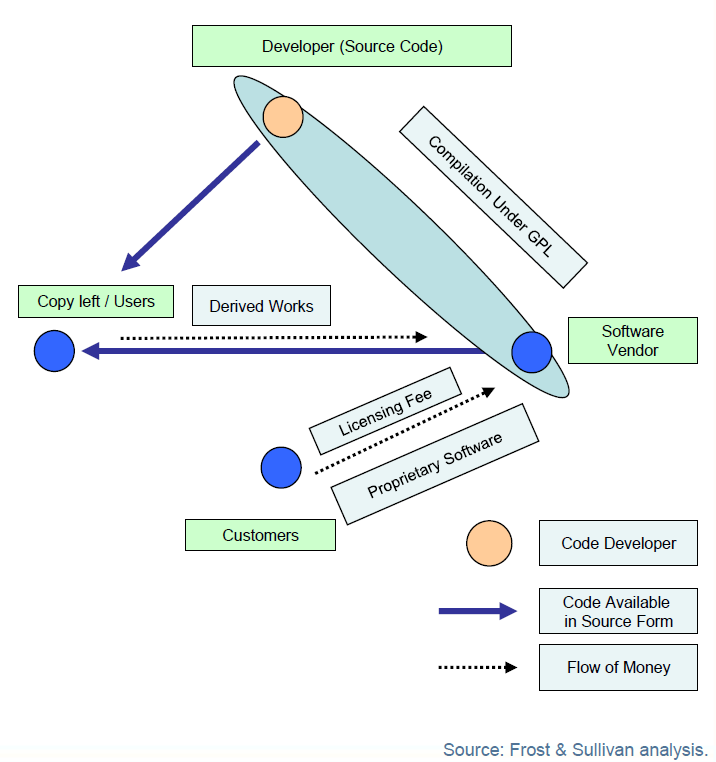
\includegraphics[width=.94\textwidth]{Impact-img1.png}}
%  \caption{The GPL Model}\label{fig:gpl-model}
% \end{figure}

% \begin{figure}[ht]\centering
%  \fbox{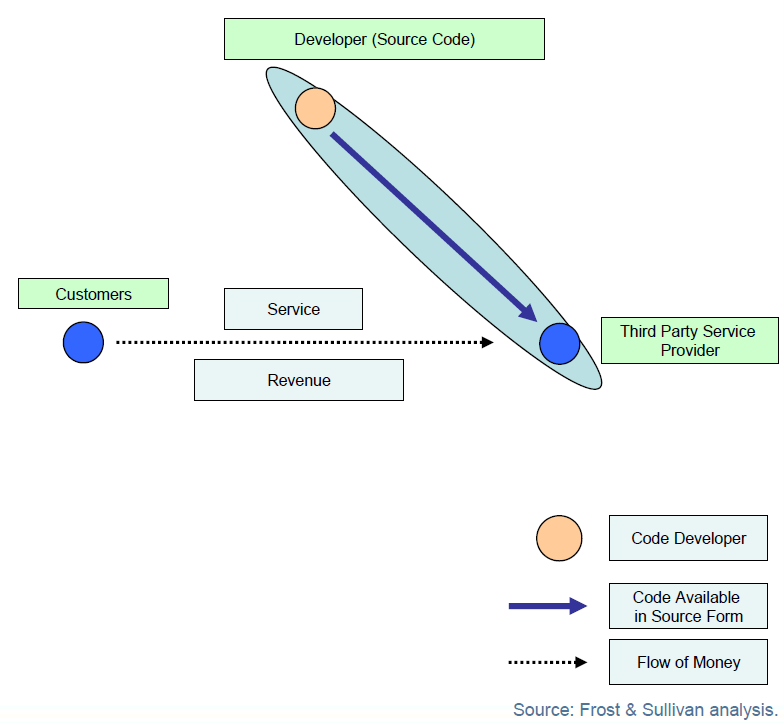
\includegraphics[width=.94\textwidth]{Impact-img2.png}}
%  \caption{The Third-Party Services Model}\label{fig:tps-model}
% \end{figure}

% \begin{compactenum}
% \item The \textbf{GPL model} (see Figure~\ref{fig:gpl-model}): With this model, the vendor
%   is required to make the new code available in source form but it can choose to keep the
%   new code as proprietary and charge for that proprietary software.  The vendor can
%   provide the code commercially as part of a larger platform (hardware/software product)
%   for which the companies receives revenue (license fee for the code + fees for technical
%   support, updates and upgrades).
% \item The \textbf{Third Party Service Model} (see Figure~\ref{fig:tps-model}) Many users
%   may be willing to employ a third party service for distribution, modifications
%   (debugging) and other support.
% \end{compactenum}

\eucommentary{
Where relevant, include information on how the participants will manage
the research data generated and/or collected during the project, in
particular addressing the following issues: What types of data will the
project generate/-collect? What standards will be used? How will this
data be exploited and/or shared/made accessible for verification and
re-use (If data cannot be made available, explain why)? How will this
data be curated and preserved?}

\TOWRITE{E.S. – Nicolas}{, ici je ne peux pas  écrire à ta place. Il faut juste que
tu répondes précisément aux questions posées ci-dessus.}

%Open source software.
%
%
%All software used and/or generated by the project will be Open Source.
%This is a deliberate choice of the project consortium, as commercial
%licenses (and patents) on this type of software only creates barriers
%in our scientific domain.
%
%Benefits of Open Source:
%
%Acquisition and Costs: lower costs, easy access to the infrastructure,
%lower risks of proprietary lock-in
%
%Flexibility: picking up from Open Source projects, reduces dependence on
%supplier, ability to view and modify the source code. Allows peer
%reviewed modifications, community discussions. Open Source provides the
%customer/end user the opportunity to innovate
%
%Support: from developer community.
%
%Besides being cost effective, Open Source software fosters
%reuse, reliability, flexibility, and interoperability.
%
%A consortium agreement will be established to manage ownership and
%access to key knowledge, including software generated by the project.

{\bf Open access policy and data protection.} OpenDreamKit will participate in the Open Research Data Pilot and is fully committed to ensure the open access of relevant project results and data. The consortium will comply with the Guidelines on Open Access to Scientific Publications and Research Data in Horizon 2020. 

The ambitious and interdisciplinary objectives of the project will result in the production of vast amount of research data (we refer to Figure \ref{fig:thebigpicture} and the corresponding subsection for more details). The primary results of the project are expected to take the form of an open-source software, which will be available through the project website and publicly available repositories. Moreover, as the project strives towards efficient integration and representation of various research data and reproducibility of the research results, which represents naturally a challenge, the project will generate a detailed description of the data sources with specifics pertaining to data management (metadata standards, policies for access and sharing and for reuse and distribution, plans for archival and preservation, with accompanying deadlines). This information will be presented in the Data Management Plan, to be delivered within the first six months after the project start and subsequently updated throughout. 

All scientific publications produced in the framework of the project will be either published in open access journals or self-archived using research data repositories. In addition, we will make all experimental data needed to reproduce/validate the results from scientific publications available through research data repositories (e.g. ZENODO, OpenAIRE). 

{\bf Intellectual Property Rights Management.} IPR management will be described in detail in the Consortium Agreement (CA), which will describe all issues regarding the IPR, confidentiality, know-how, rights on exploitation, the rights and obligations of the each partner. The CA will be prepared by the Coordinator, and then signed by all partners before the start of the project. 

Access rights to foreground and background needed for the execution of the project shall be deemed granted, on a royalty-free basis, as of the date of the grant agreement entering into force. Methodology, documents, know-how, software, and tools will be available to all in order to achieve the project objectives during the project lifetime. 

Most of the project results will have joint ownership due to a highly collaborative nature of the project. The CA will specify the terms of the resulting joint ownership, i.e., assignment of shares between joint owners, conditions of use, exploitation and management of jointly used IP. 

The CA will also outline rules for publication procedures to ensure that IP can be protected while minimising publication delay.

The costs related to IPR (including those related to protecting results) and dissemination (i.e., 'gold' open access publications) are included in the project budget of each participating organisation. 

\subsubsection{Communication Activities}
\label{subsubsect:communication}

\eucommentary{Describe the proposed communication measures for promoting the
project and its findings during the period of the grant. Where appropriate
these measures should include social media and public events with user
participation. Measures should be proportionate to the scale of the project,
with clear objectives. They should be tailored to the needs of various audiences,
including groups beyond the project's own community. Where relevant, include
measures for public/societal engagement on issues related to the project.}

Our intention is to increase the attractiveness of mathematics among young generation and females in particular as well as to improve the impact and maximise the visibility of the project activities on the entire VRE ecosystem. The following strategic access points will be used to maximise visibility:

\begin{compactenum}
\item An online presence that explains the OpenDreamKit concept and its applicability in layman's terms and offers significant information (website, social networks, Youtube, press releases).
\item Collaboration with other relevant European and national projects (existing and new ones). We refer to Section \ref{linked-projects} for more details on the linked research and innovation activities.  Presentation of the project results on the annual event 'Worldwide meetings of the free software.' 
\item Collaboration with European and national mathematical societies, e.g., European Mathematical Society, European Women in Mathematics.
\item Presentations/demonstrations at partner institution-specific, locally organised 'science holiday' and 'days of science'.
\item Popularisation papers and communication events addressed to people interested by ICT. 
\item Involvement in workshops / conferences on e-infrastructures and broad mathematical topics, e.g., Swiss Numerical Analysis Day.
\end{compactenum}
%%% Local Variables:
%%% mode: latex
%%% TeX-master: "proposal"
%%% End:

%  LocalWords:  eucommentary programme subsubsection tablehead longtable hline sur est
%  LocalWords:  e-infrastracture sémantique données amont j'ai mal si répond vraiment ce
%  LocalWords:  critère Systeme flushleft arraybslash Ergonomie il faut réflechir façon
%  LocalWords:  rendre l'outil attractif jeune génération génération des chercheurs va je
%  LocalWords:  définir donc terme Réfléchis possibilité tablettes mais aussi l'enseigner
%  LocalWords:  intéressante textgreater partie suivante demande elle ne serait mieux que
%  LocalWords:  unauthorised Maximise subsubsect organisational Pycon IPython Economie tu
%  LocalWords:  Standartisation Logiciel Libre includegraphics Impact-img1.png peux emph
%  LocalWords:  Impact-img2.png écrire répondes précisément posées ci-dessus TOWRITE fbox
%  LocalWords:  Simula Valeriya textwidth textwidth textbf compactenum longtable Jupyter
%  LocalWords:  organisation organise neighbouring Standartization programmes gpl-model
%  LocalWords:  tps-model thebigpicture Popularisation virtualised organisations Logilab
%  LocalWords:  organisations summarise organising capitalise realising minimising
%  LocalWords:  organised
\newpage
\chapter{Ethical Issues}\label{chap:ethical}
\begin{todo}{from the proposal template}
  Describe any ethical issues that may arise in the project. In particular, you should
  explain the benefit and burden of the experiments and the effects it may have on the
  research subject. Identify the countries where research will be undertaken and which
  ethical committees and regulatory organisations will need to be approached during the
  life of the project.

  Include the Ethical issues table below.  If you indicate YES to any issue, please
  identify the pages in the proposal where this ethical issue is described. Answering
  'YES' to some of these boxes does not automatically lead to an ethical review1.  It
  enables the independent experts to decide if an ethical review is required. If you are
  sure that none of the issues apply to your proposal, simply tick the YES box in the last
  row.
\end{todo}

\begin{small}
\begin{tabular}{|p{1em}p{11cm}|l|l|}\hline
  \multicolumn{2}{|l|}{\cellcolor{lightgray}{\strut}} & 
  \cellcolor{lightgray}{YES} & 
  \cellcolor{lightgray}{PAGE}\\\hline 
  \multicolumn{2}{|l|}{\bf{Informed Consent}} & & \\\hline
  & Does the proposal involve children?  & & \\\hline
  & Does the proposal involve patients or persons not able to give consent? & & \\\hline
  & Does the proposal involve adult healthy volunteers? & & \\\hline
  & Does the proposal involve Human Genetic Material? & & \\\hline
  & Does the proposal involve Human biological samples? & & \\\hline
  & Does the proposal involve Human data collection? & & \\\hline
  \multicolumn{2}{|l|}{\bf{Research on Human embryo/foetus}}  & & \\\hline
  & Does the proposal involve Human Embryos? & & \\\hline
  & Does the proposal involve Human Foetal Tissue / Cells? & & \\\hline
  & Does the proposal involve Human Embryonic Stem Cells? & & \\\hline
  \multicolumn{2}{|l|}{\bf{Privacy}} & & \\\hline
  & Does the proposal involve processing of genetic information 
         or personal data (eg. health, sexual lifestyle, ethnicity, 
         political opinion, religious or philosophical conviction)  & & \\\hline 
  & Does the proposal involve tracking the location or observation 
         of people? & & \\\hline 
  \multicolumn{2}{|l|}{\bf{Research on Animals}} & & \\\hline 
  & Does the proposal involve research on animals? & & \\\hline 
  & Are those animals transgenic small laboratory animals? & & \\\hline 
  & Are those animals transgenic farm animals? & & \\\hline 
  & Are those animals cloned farm animals? & & \\\hline 
  & Are those animals non-human primates?  & & \\\hline 
  \multicolumn{2}{|l|}{\bf{Research Involving Developing Countries}} & & \\\hline 
  & Use of local resources (genetic, animal, plant etc) & & \\\hline 
  & Benefit to local community (capacity building 
         i.e. access to healthcare, education etc) & & \\\hline 
  \multicolumn{2}{|l|}{\bf{Dual Use}} & & \\\hline 
  & Research having direct military application  & & \\\hline 
  & Research having the potential for terrorist abuse & & \\\hline 
  \multicolumn{2}{|l|}{\bf{ICT Implants}} & & \\\hline 
  & Does the proposal involve clinical trials of ICT implants?  & & \\\hline 
  \multicolumn{2}{|l|}{\bf\footnotesize{I CONFIRM THAT NONE OF THE ABOVE ISSUES APPLY TO MY PROPOSAL}} 
      & &\cellcolor{lightgray}{} \\\hline 
\end{tabular}
\end{small}

\section{Personal Data}

\end{proposal}
\end{document}

%%% Local Variables: 
%%% mode: LaTeX
%%% TeX-master: t
%%% End: 

% LocalWords:  efo efoRM baz bazRM miko acrolong ntelligent iting pn pnlong
% LocalWords:  textsc newpage compactht texttt euproposal.cls callname callid
% LocalWords:  challengeid objectiveid outcomeid tableofcontents
